% uid: ""
% school: "college"
% level: "7eme"
% chapter: "التناظر المحوري"
% chapter_slug: "symetrie-axiale"
% title: "أتمم الشكل : محور مائل"
% difficulty: "Facile"
% tags: ["symetrie-axiale", "quadrillage", "axe-oblique", "construction"]
% provenance: "own"
% batch: "2026-11-27-symetrie-axiale-7eme"
% Exercice 7/10 de la série 7ème « التناظر المحوري » (statement + \axsol + solution). Compiler avec XeLaTeX + axiomath.sty (+ axiomaths-logo.png).
\documentclass[12pt,a4paper]{article}
\usepackage[level=7b,color=0F766E]{axiomath}
\newcommand{\cm}{\,\mathrm{cm}}
\axsetup{title={التناظر المحوري}, corrige}

\begin{document}

\begin{corr}[title={أتمم الشكل : محور مائل}, stars=2, source={Axiomaths}]
المستقيم $\Delta$ يمرّ من رؤوس مربعات الشبكة (قطرها).
\begin{center}
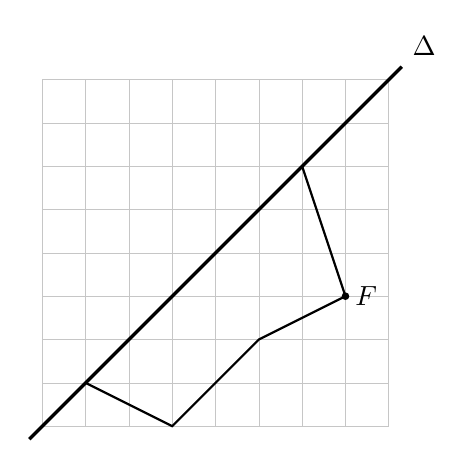
\begin{tikzpicture}[scale=0.55]
  \draw[gray!45,very thin] (0,0) grid (8,8);
  \draw[very thick] (-0.3,-0.3)--(8.3,8.3) node[above right] {$\Delta$};
  \draw[thick] (1,1)--(3,0)--(5,2)--(7,3)--(6,6);
  \fill (7,3) circle (2.5pt) node[right] {$F$};
\end{tikzpicture}
\end{center}
\begin{enumerate}
  \item أتمم الشكل بحيث يكون $\Delta$ محور تناظر له.
  \item عيّن النقطة $F'$ مناظرة $F$ بالنسبة إلى $\Delta$.
  \item تحقق على الشبكة أن منتصف $[FF']$ ينتمي إلى $\Delta$.
\end{enumerate}
\axsol
\begin{enumerate}[itemsep=14pt]
  \item\leavevmode
  \begin{prop}[محور مائل على الشبكة]
  $(FF')$ عمودي على $\Delta$ : ننتقل على \ib{القطر الآخر للمربعات}. نعدّ المربعات حتى نصل إلى $\Delta$ ، ثم \ib{نواصل بنفس العدد} في الجهة الأخرى.
  \end{prop}
  نطبّق ذلك على كل رأس من رؤوس الخط المنكسر :
  \begin{itemize}
    \item الرأسان على $\Delta$ (في الأسفل وفي الأعلى) هما مناظرا نفسيهما.
    \item كل رأس آخر نبني مناظره بالطريقة السابقة، ثم نصل النقاط بنفس الترتيب.
  \end{itemize}
  \begin{center}
  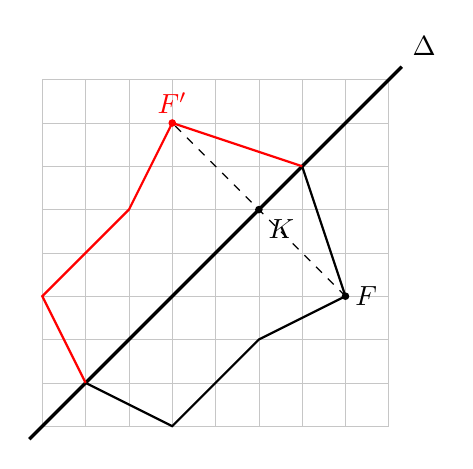
\begin{tikzpicture}[scale=0.55]
    \draw[gray!45,very thin] (0,0) grid (8,8);
    \draw[very thick] (-0.3,-0.3)--(8.3,8.3) node[above right] {$\Delta$};
    \draw[thick] (1,1)--(3,0)--(5,2)--(7,3)--(6,6);
    \draw[thick,red] (1,1)--(0,3)--(2,5)--(3,7)--(6,6);
    \draw[dashed] (7,3)--(3,7);
    \fill (7,3) circle (2.5pt) node[right] {$F$};
    \fill[red] (3,7) circle (2.5pt) node[above] {$F'$};
    \fill (5,5) circle (2.5pt) node[below right] {$K$};
  \end{tikzpicture}
  \end{center}
  \item من $F$ ننتقل على قطر المربعات (إلى اليسار وإلى الأعلى) : بعد قطرين نصل إلى $\Delta$ في النقطة $K$.

  نواصل قطرين آخرين في نفس الاتجاه فنجد \ib{$F'$}.
  \item من $F$ إلى $K$ : قطران، ومن $K$ إلى $F'$ : قطران. إذن $KF=KF'$ و $F$ و $K$ و $F'$ على استقامة واحدة : $K$ منتصف $[FF']$.

  و $K$ تنتمي إلى $\Delta$ : \ib{منتصف $[FF']$ ينتمي إلى $\Delta$}، كما يقتضيه التعريف.
\end{enumerate}
\end{corr}

\end{document}
